% Appendix

\chapter*{Appendix A} % Main appendix title

\label{AppendixA} % Change X to a consecutive letter; for referencing this appendix elsewhere, use \ref{AppendixX}

\begin{figure}
      \centering
      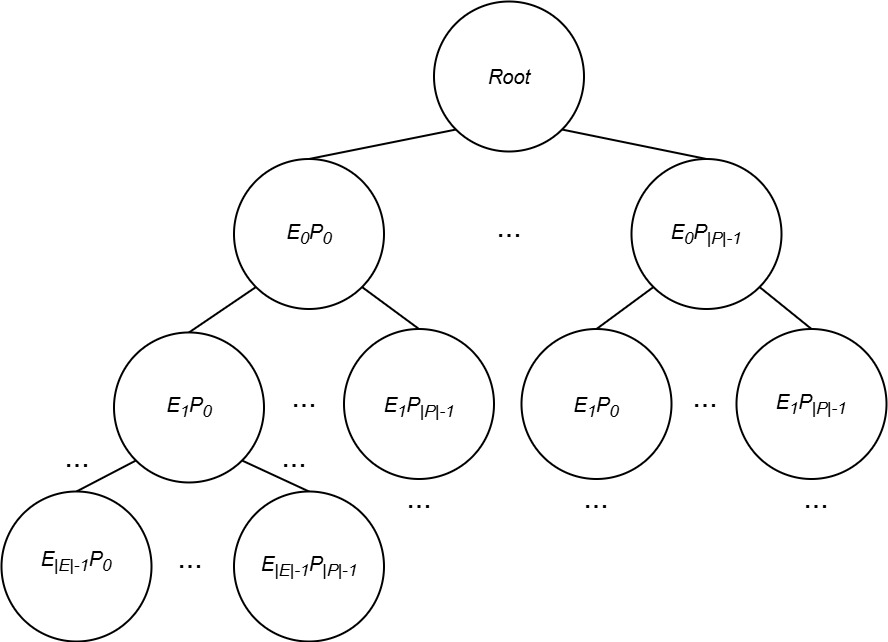
\includegraphics[width=0.7\columnwidth]{AppendixA/tree.jpg}
      \caption[Proposed \ac{mcts} tree]
      {Proposed \ac{mcts} tree}
      \label{fig:tree}
\end{figure}


\begin{figure}
      \centering
      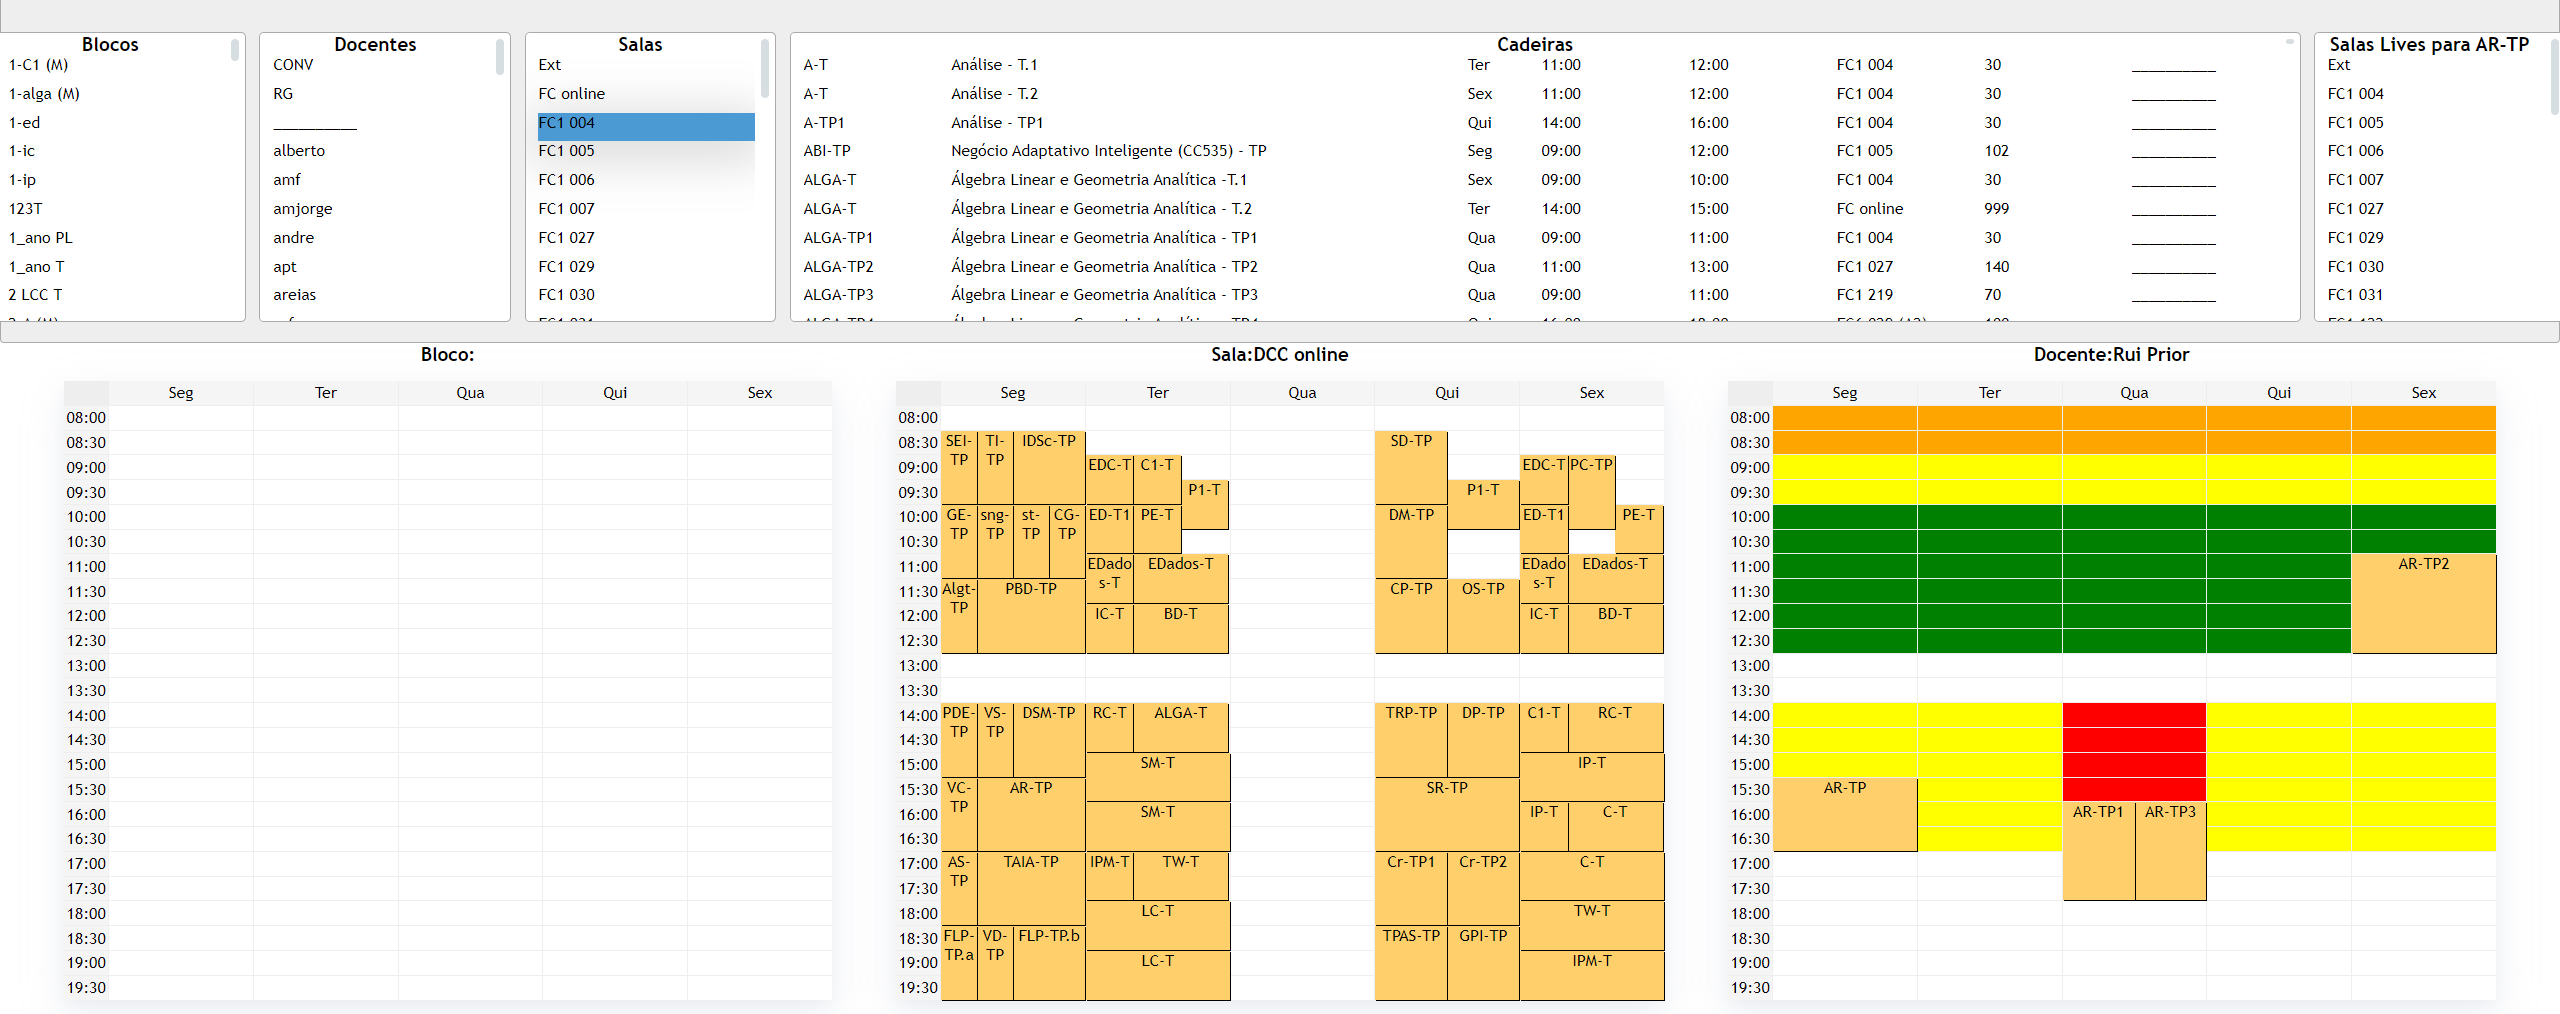
\includegraphics[width=1.0\columnwidth]{AppendixA/previous_work.png}
      \caption[Previous work interface]
      {Previous work interface}
      \label{fig:previous_work_interface}
\end{figure}

\begin{figure}
      \centering
      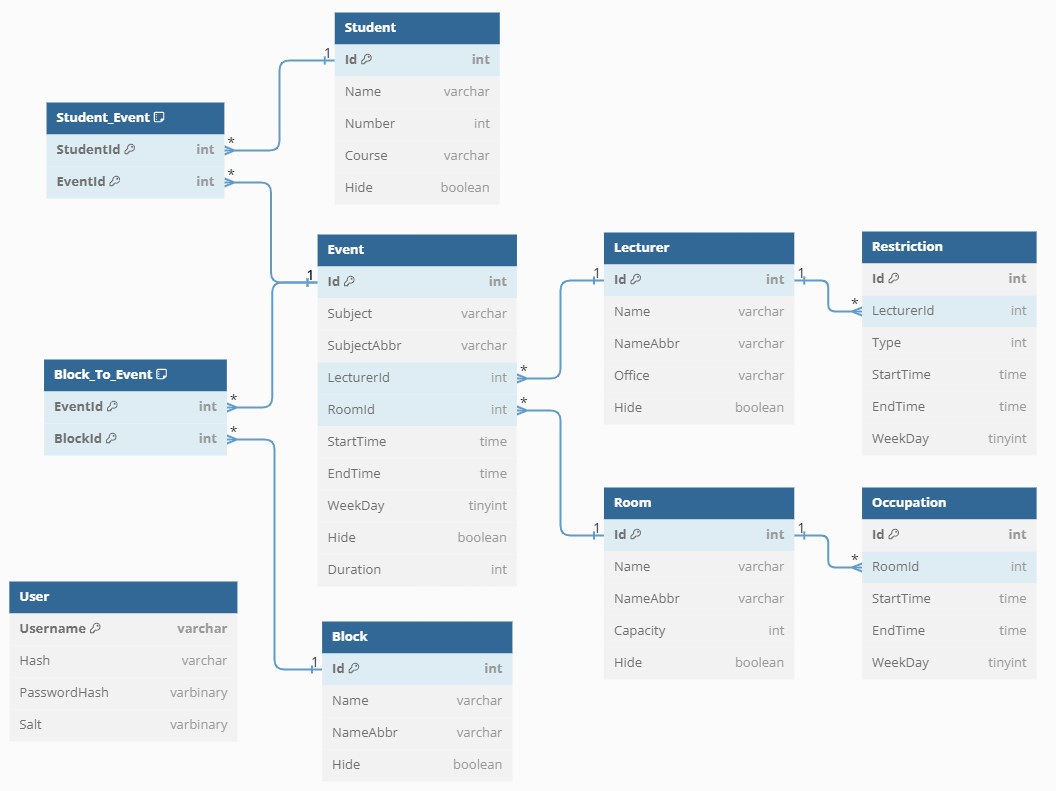
\includegraphics[width=1.0\columnwidth]{AppendixA/uml.png}
      \caption[Previous work UML]
      {Previous work UML}
      \label{fig:previous_work_uml}
\end{figure}


\begin{algorithm}
\caption{Simulation}\label{simulation}
\begin{algorithmic}[1]
\Function{SIMULATION}{start\_time, time\_limit}
    \State assigned\_events $\gets$ current\_node.path.\textit{copy}()
    \State unassigned\_events $\gets$ \textit{set}()
    \State remaining\_events $\gets$ \textit{sorted}(events[current\_node.\textit{depth}():], 
    \Statex \hspace{3cm} \textbf{key} = $\lambda$ event: (event["Id"] \textbf{in} previous\_unassigned\_events, event["Priority"], \textit{random.random()}), 
    \Statex \hspace{3cm} \textbf{reverse} = True)
    \\
    \For{\textbf{each} $i, event$ \textbf{in} \textit{enumerate}(remaining\_events)}
        \State best\_room\_and\_period $\gets$ \textit{find\_best\_room\_and\_period}()
        \If{best\_room\_and\_period exists}
            \State event["RoomId"], event["WeekDay"], event["Timeslot"] $\gets$ best\_room\_and\_period
            \State assigned\_events[event["Id"]] $\gets$ event
        \Else
            \State previous\_unassigned\_events.\textit{add}(event["Id"])
            \State unassigned\_events.\textit{add}(event["Id"])
        \EndIf
    \EndFor
    \\
    \State hard\_penalty\_result, soft\_penalty\_result $\gets$ \textit{evaluate\_timetable}(assigned\_events, unassigned\_events)
    \\
    \State \textit{update\_penalties}(soft\_penalty\_result, hard\_penalty\_result)
    \\
    \If{(hard\_penalty\_result $>$ global\_best\_hard\_penalty) \textbf{or} (hard\_penalty\_result = global\_best\_hard\_penalty \textbf{and} soft\_penalty\_result $>$ global\_best\_soft\_penalty)}
        \State global\_best\_hard\_penalty $\gets$ hard\_penalty\_result
        \State global\_best\_soft\_penalty $\gets$ soft\_penalty\_result
        \State \textbf{with} \textit{open}(output\_filename, 'w') \textbf{as} file:
            \State \hspace{1cm} \textit{write\_best\_simulation\_result\_to\_file}(\textit{list}(assigned\_events.values()), file)
        \If{\textit{len}(unassigned\_events) $==$ 0 \textbf{and} hard\_penalty\_result $==$ 0 \textbf{and} soft\_penalty\_result $\neq$ 0}
            \State global\_best\_soft\_penalty $\gets$ hill\_climber.\textit{run\_hill\_climbing}(assigned\_events, 
            \Statex \hspace{3cm} events[current\_node.\textit{depth}()]["Id"], 
            \Statex \hspace{3cm} global\_best\_soft\_penalty, start\_time, time\_limit)
            \State \textit{update\_penalties}(global\_best\_soft\_penalty)
        \EndIf
    \EndIf
    \\
    \State simulation\_result\_hard $\gets$ \textit{normalize\_hard}(current\_node.best\_hard\_penalty)
    \State simulation\_result\_soft $\gets$ \textit{normalize\_soft}(current\_node.best\_soft\_penalty)
    \\
    \State \Return simulation\_result\_hard, simulation\_result\_soft
\EndFunction
\end{algorithmic}
\end{algorithm}

\begin{algorithm}
\caption{Run Hill Climbing}\label{run_hill_climbing}
\begin{algorithmic}[1]
\Function{RUN\_HILL\_CLIMBING}{best\_timetable, start\_key, best\_result\_soft, start\_time, time\_limit}
    \State best\_result\_soft $\gets$ best\_result\_soft
    \State neighborhoods $\gets$ [(\textit{period\_move}, 1), (\textit{room\_move}, 1), (\textit{event\_move}, 1), (\textit{room\_stability\_move}, 0.7), (\textit{min\_working\_days\_move}, 0.5), (\textit{curriculum\_compactness\_move}, 0.7)]
    \\
    \State idle\_iterations $\gets$ 0
    \\
    \While{idle\_iterations $<$ HC\_IDLE \textbf{and} (time.time() - start\_time $\leq$ time\_limit)}
        \State (current\_neighborhood, \_) \gets$ weighted random choice from neighborhoods
        \\
        \State unscheduled\_events $\gets$ \textit{dict\_slice}(best\_timetable, start\_key)
        \\
        \State modified\_timetable $\gets$ current\_neighborhood(best\_timetable, unscheduled\_events)
        \\
        \If{modified\_timetable is \textbf{None}}
            \State idle\_iterations $\gets$ idle\_iterations + 1
            \State \textbf{continue}
        \EndIf
        \\
        \State result $\gets$ \textit{evaluate\_timetable}(modified\_timetable)
        \\
        \If{result is not \textbf{None}}
            \If{result $>$ best\_result\_soft}
                \State best\_result\_soft $\gets$ result
                \State best\_timetable $\gets$ modified\_timetable
                \State \textit{write\_simulation\_results}(output\_filename, best\_timetable.values(), start\_time, 0, result)
                \If{result $=$ 0}
                    \State \Return 0
                \EndIf
                \State idle\_iterations $\gets$ 0
            \Else
                \State \textit{revert\_changes}(best\_timetable)
                \State idle\_iterations $\gets$ idle\_iterations + 1
            \EndIf
        \Else
            \State \textit{revert\_changes}(best\_timetable)
            \State idle\_iterations $\gets$ idle\_iterations + 1
        \EndIf
    \EndWhile
    \\
    \State \Return best\_result\_soft
\EndFunction
\end{algorithmic}
\end{algorithm}
